\begin{frame}
\frametitle{Work of Master's Program}
\begin{enumerate}
    \small \item \small Study of problems in Science and Engineering needing Computational Simulation and performance optimization. 
    \begin{itemize} 
    \item \small Performance Tuning the Lattice-Boltzmann for Simulation of Blood Flow of Human Heart.
    \item \small Computational simulation for Biofuels. 
    \end{itemize}
    \item \small Parallel Sorting Pattern 
    \item \small Correlation between NAS Parallel Benchmarks and Parallel Patterns for Improved Benchmarking and Parallel Application development. 
    \item \small MPI+MPI Programming Model 
\end{enumerate}
\end{frame}

%\begin{frame}{Applications in Renewable Energy} 
%\end{frame}

\begin{frame}{Performance Tuning the Lattice-Boltzmann for Simulation of Blood Flow of Human Heart\footnote{\tiny {A. Randles, V. Kale, J. Hammond, W. Gropp and E. Kaxiras} {\it Performance Analysis of the Lattice Boltzmann Model Beyond Navier-Stokes.} IPDPS 2013.}}

\begin{columns} 
\column{0.2\columnwidth}
\begin{figure}[ht!]
%includegraphics[scale=0.1]{images/Fluid-density-in-the-aorta.png}
\end{figure}

\column{0.8\columnwidth}
\begin{itemize}
\footnotesize  \item \footnotesize present a performance study of the higher-order models as compared to the traditional ones, on both the IBM Blue Gene/P and Blue Gene/Q architectures. 
\item \footnotesize Study the tradeoffs of many optimizations methods such as the use of deep halo level ghost cells that, alongside hybrid programming models, reduce the impact of extended models and enable efficient modeling of extreme regimes of computational fluid dynamics. 
\end{itemize} 
\end{columns}

\begin{figure}[ht!]
\centering
%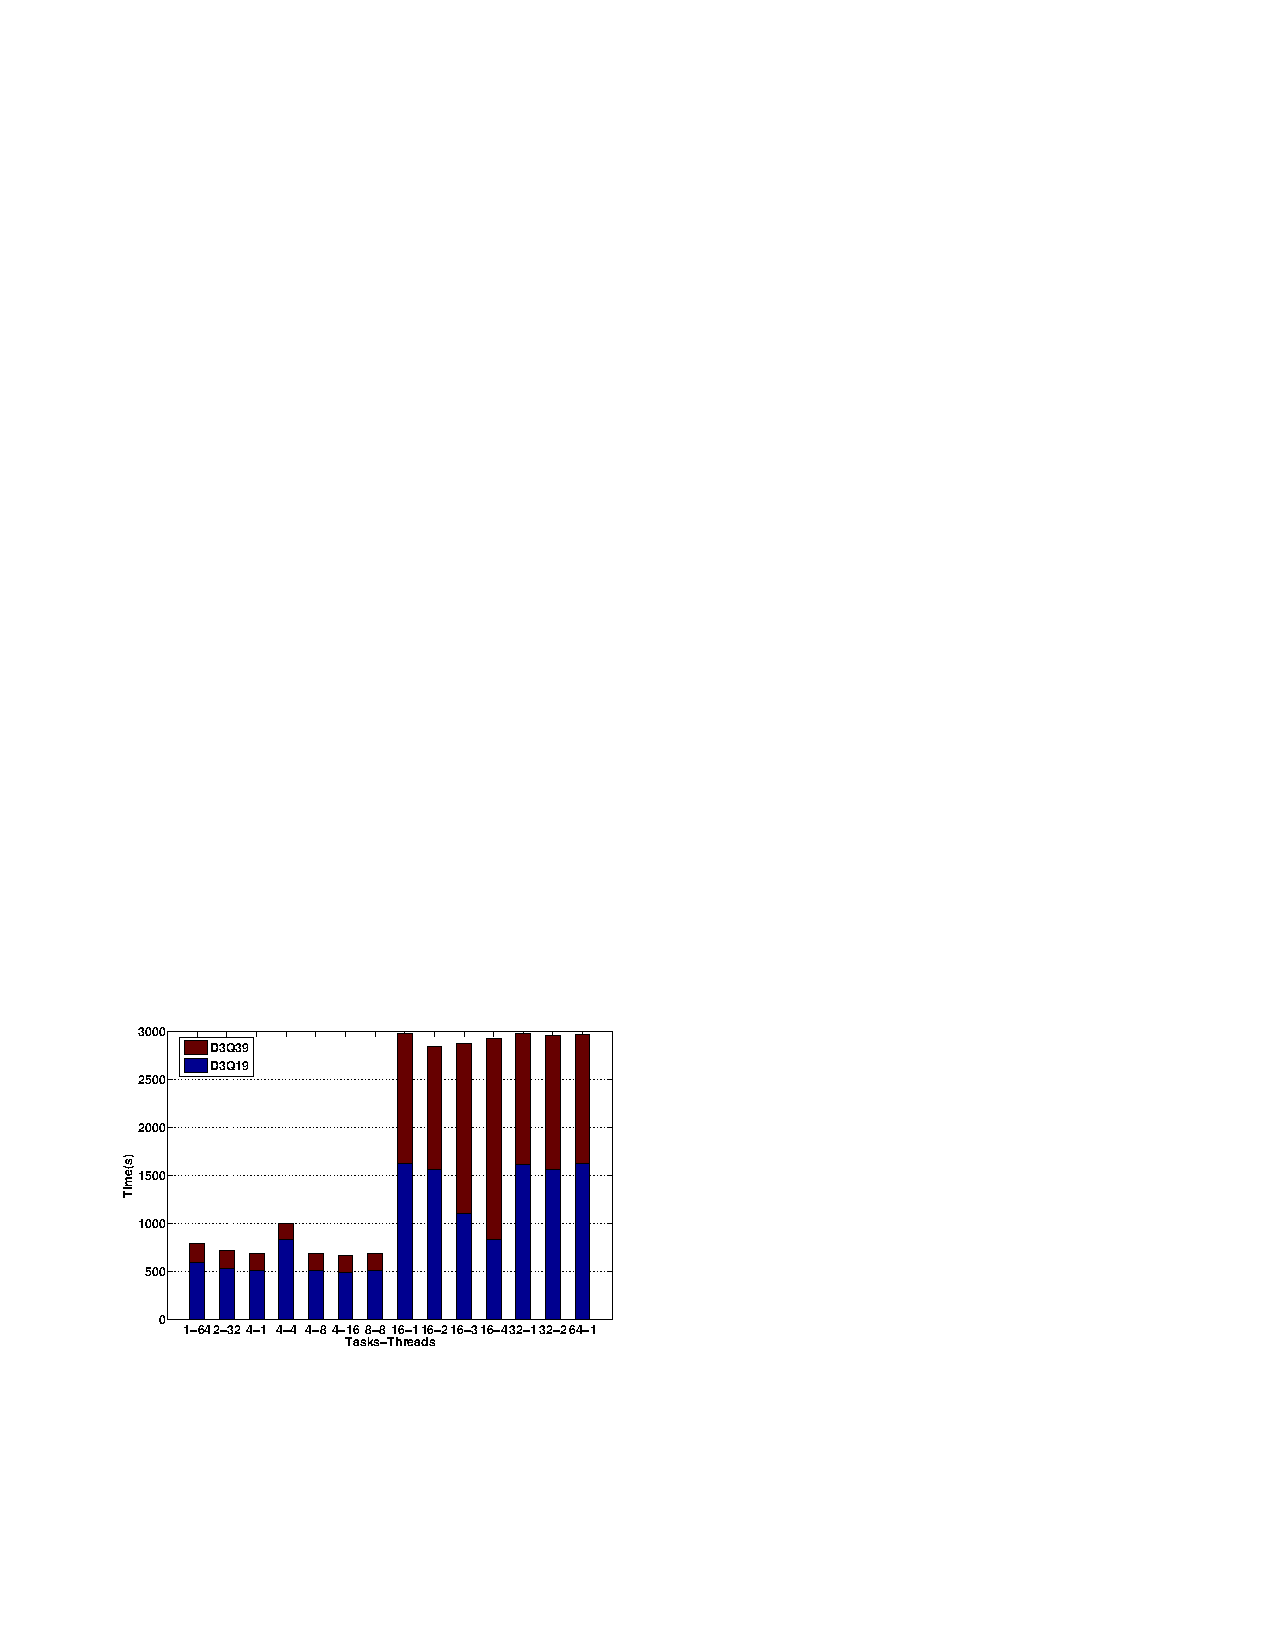
\includegraphics[scale=0.49]{plots/TasksThreadsLBM_BGQresults}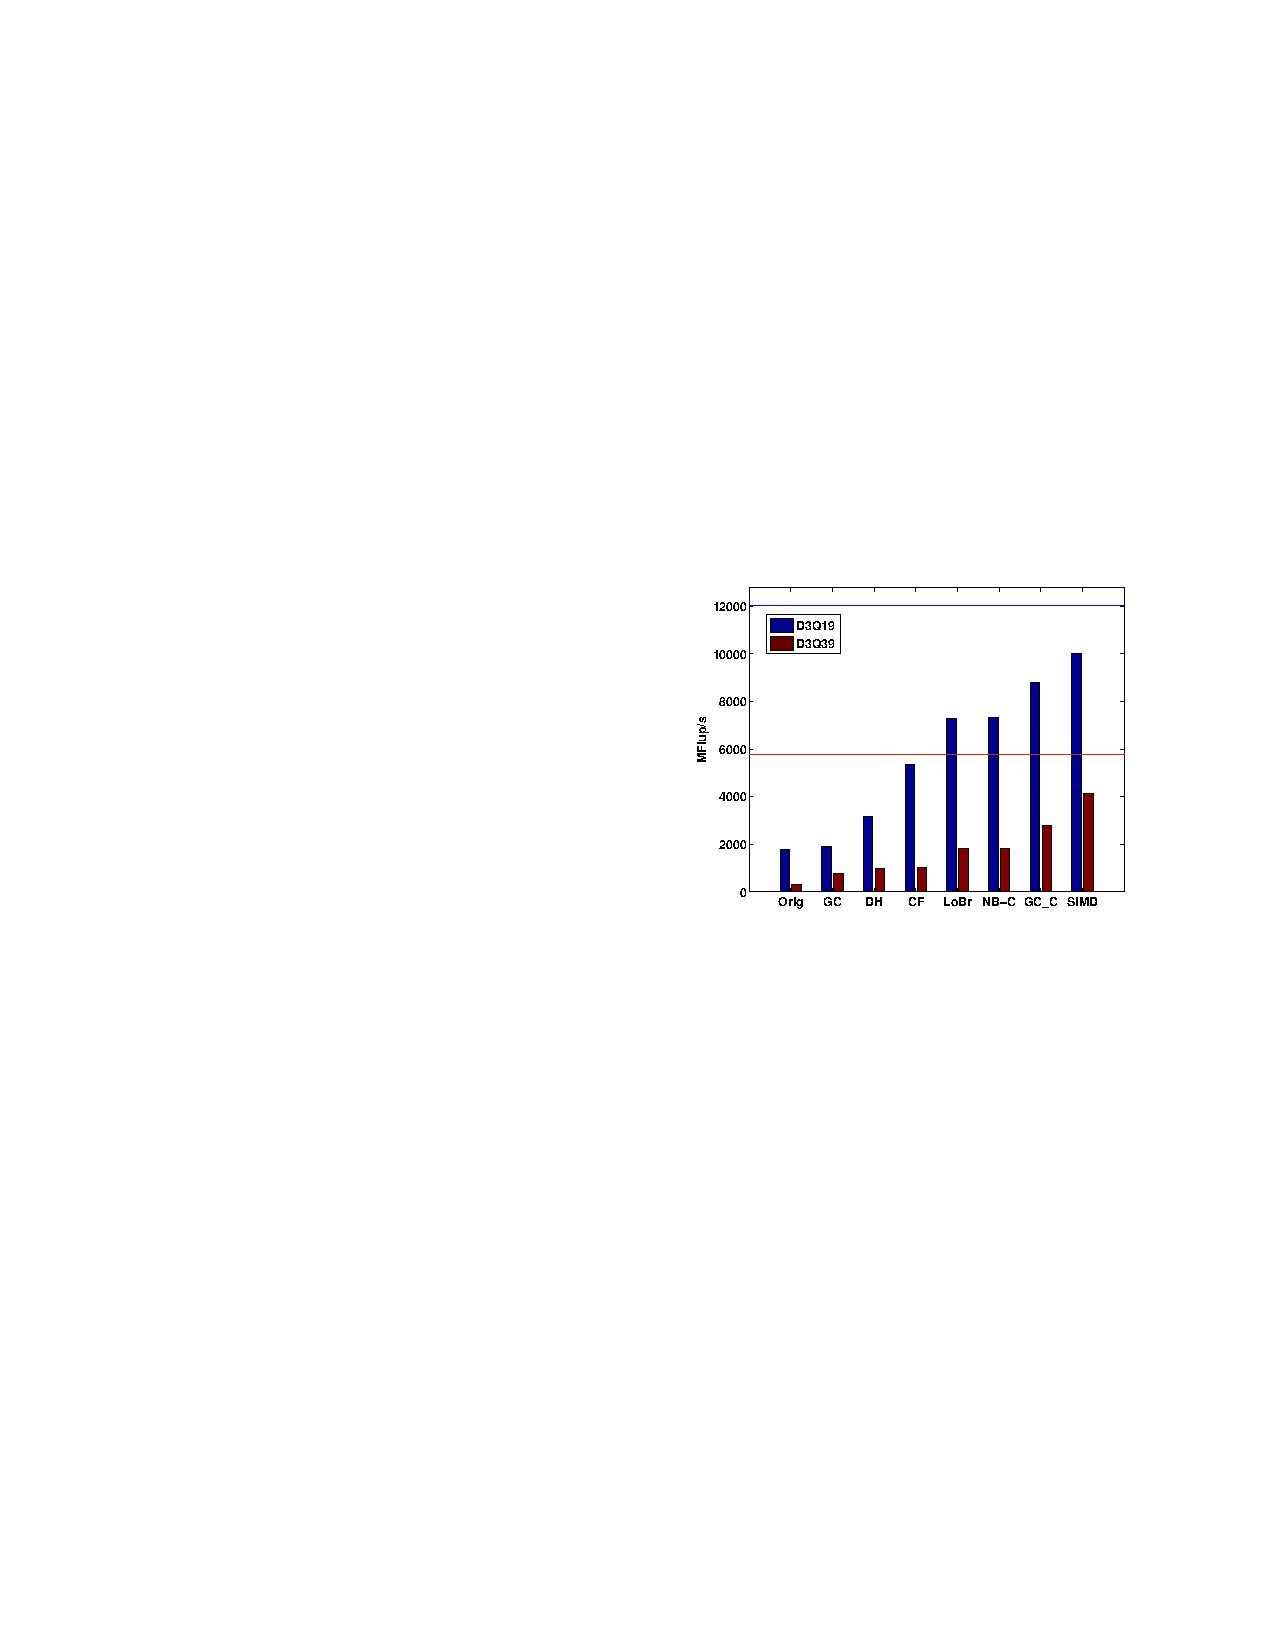
\includegraphics[scale=0.49]{plots/LBM_PerfOpts_BGQ}
\end{figure}

%\column{0.5\columnwidth} 
%\end{columns}
\end{frame}

\begin{frame}{Designing Parallel Sorting Algorithms: A Patterns Approach\footnote{\tiny Kale, V., Solomonik, E. {\it Parallel Sorting Pattern} ParaPLOP 2010. July 2010.}}
\begin{itemize}
    \footnotesize \item \footnotesize A large number of parallel applications contain a computationally intensive phase in which a large list of elements must be ordered based on some common attribute of the elements.
    \item \footnotesize How do we sort a sequence of elements on multiple processing units so as to minimize redistribution of keys while allowing processing units to do independent sorting work.
    \item \footnotesize Show general method to design a parallel sorting algorithm 
     \item \footnotesize Design and assess theoretical performance of four parallel sorting algorithms: quicksort, radix sort, sample sort, merge sort.
\end{itemize}
\end{frame}

\begin{frame}{NAS Parallel Benchmarks $\curvedrightleft$ Parallel Design Patterns\footnote{\tiny Kale, V. {\it Correlations between Parallel Patterns and Multi-core Benchmark.} IWMSE '10. May 2010.}} 

{\footnotesize The NAS LU benchmark is a Gauss-Seidel kernel, used for applications involving simulation of heat dissipation and fluid dynamics.}
\begin{itemize}
   \footnotesize \item \footnotesize {\bf Computational Pattern:} structured grid $\rightarrow$ LU can be identified directly with a structured grid computation pattern because of border exchanges involved. 
    \item \footnotesize {\bf Structural Pattern}: iterative refinement $\rightarrow$ LU uses the iterative refinement structural pattern because of the outer loop that it iterates over until convergence. 
    \item \footnotesize {\bf Algorithmic Structure Pattern}: geometric decomposition $\rightarrow$ LU benchmark involves exchanges of data between neighboring cells in the grid; this requires the use of “halo” or ghost cells.
    \item \footnotesize {\bf Implementation Pattern}: pipeline parallelism $\rightarrow$ Processor 0 starts at the topmost row, while processor 1 starts at one timestep later, using the result of the computation of processor 0 in the first timestep. Processor 2 follows processor 1, and so on. 
    \item \footnotesize {\bf Parallel Execution Strategy Pattern}: Depends! $\rightarrow$ NAS LU  is now implemented in different programming libraries.
\end{itemize}
\end{frame}

%\begin{frame}{Towards Using and Improving the NAS Parallel Benchmarks: A Patterns Approach}
%\end{frame}
 
\begin{frame}{Auto-tuning Scientific Kernels for Emerging High-Performance Computer Architectures} 
\begin{itemize}
    \small \item \small Even with emerging cluster of SMP architectures, the MPI-everywhere model is dominant in scientific codes. 
    \item \small However, the MPI-everywhere model sacrifices efficiency advantages of shared memory multi-processor technology, particularly when scaling to millions of nodes. 
    \item \small Using our library for optimizing performance of such codes we: 
    \begin{enumerate}
      \tiny \item \tiny discuss early experiences in hybridizing scientific codes; 
      \item \tiny identify performance optimizations that take advantage of shared memory;
      \item \tiny compare initial performance results to codes using the MPI-everywhere model.
    \end{enumerate}
\end{itemize}
\end{frame}

\begin{frame}{MPI+MPI\footnote{\tiny {\it MPI + MPI: A New Hybrid Approach to Parallel Programming with MPI Plus Shared Memory.} Hoefler, T., Dinan, J., Buntinas, D., Balaji, P., Barrett, B., Brightwell, R, Gropp, W.D., Kale, V., Thakur, R.  Journal of 	Parallel Computing. 2013.}}
\vspace*{-.1in}
\begin{enumerate}
  \footnotesize \item \footnotesize \comments{Problem:} While a hybrid MPI+X parallel programming model provides flexibility and performance potential, it makes programming complex due to having to use two parallel programming systems in the same application.
%  \item \footnotesize We introduce an MPI-integrated shared-memory programming model that is incorporated into MPI through a small extension to the one-sided communication interface. 
   \item \footnotesize \comments{Technique:} MPI+MPI is an integration of an interface with MPI 3.0 one-sided semantics. 
%   \item \footnotesize We describe an implementation of the new interface in the MPICH2 and Open MPI implementations. 
   \item \footnotesize \comments{Experimental Setup:} Run a five-point stencil on a six-core 2.2 GHz AMD Opteron CPU with two MPI processes using an mpich and OpenMPI library supporting MPI+MPI
\end{enumerate}
\vspace*{-0.3in}
%\begin{columns}
%\column{0.7\columnwidth}
\begin{figure}[ht!]
\label{fig:stencilMPIMPIbgq}
  %  \centering
   % \subfloat[\tiny Communication Overhead.]{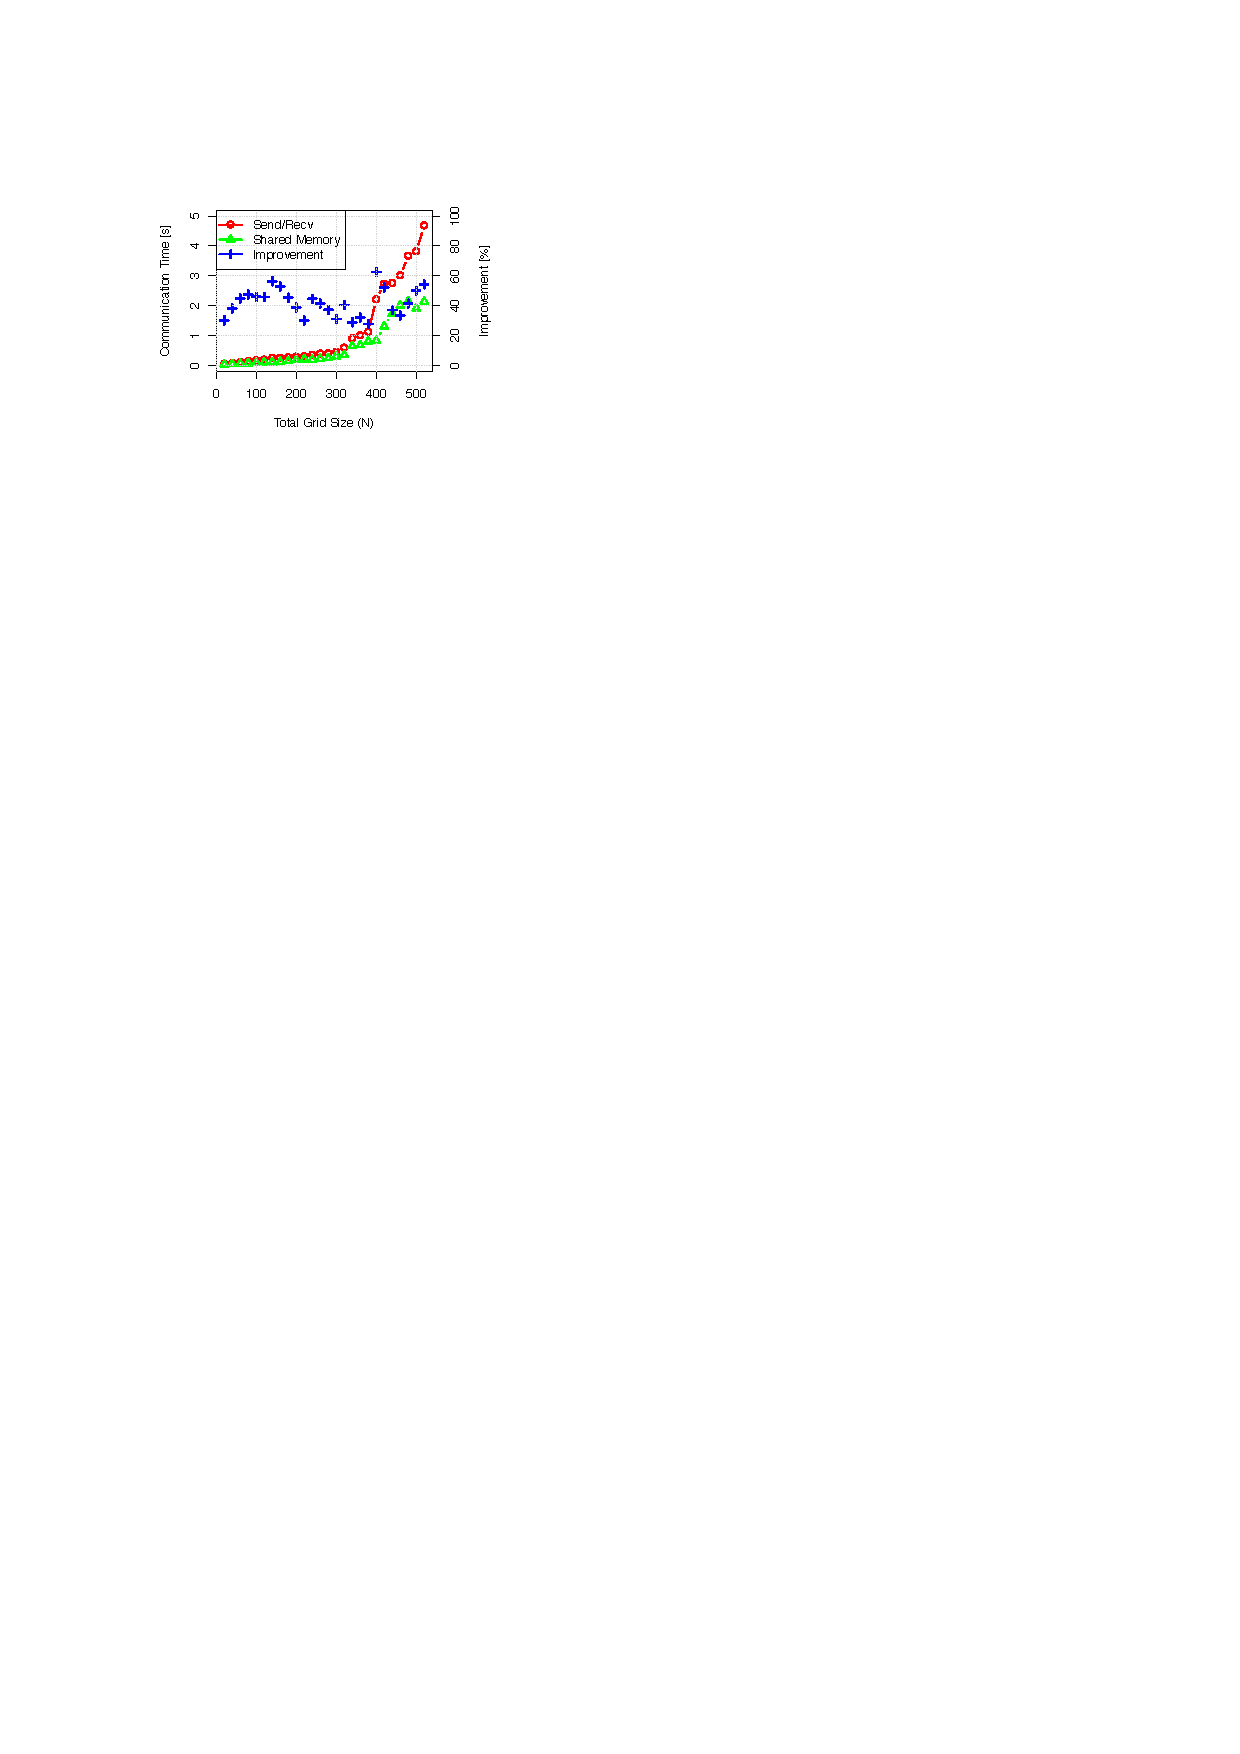
\includegraphics[scale=0.7]{./plots/Stencil_MPIMPI_CommOvhd_6core}}\subfloat[\tiny Computation Slowdown.]{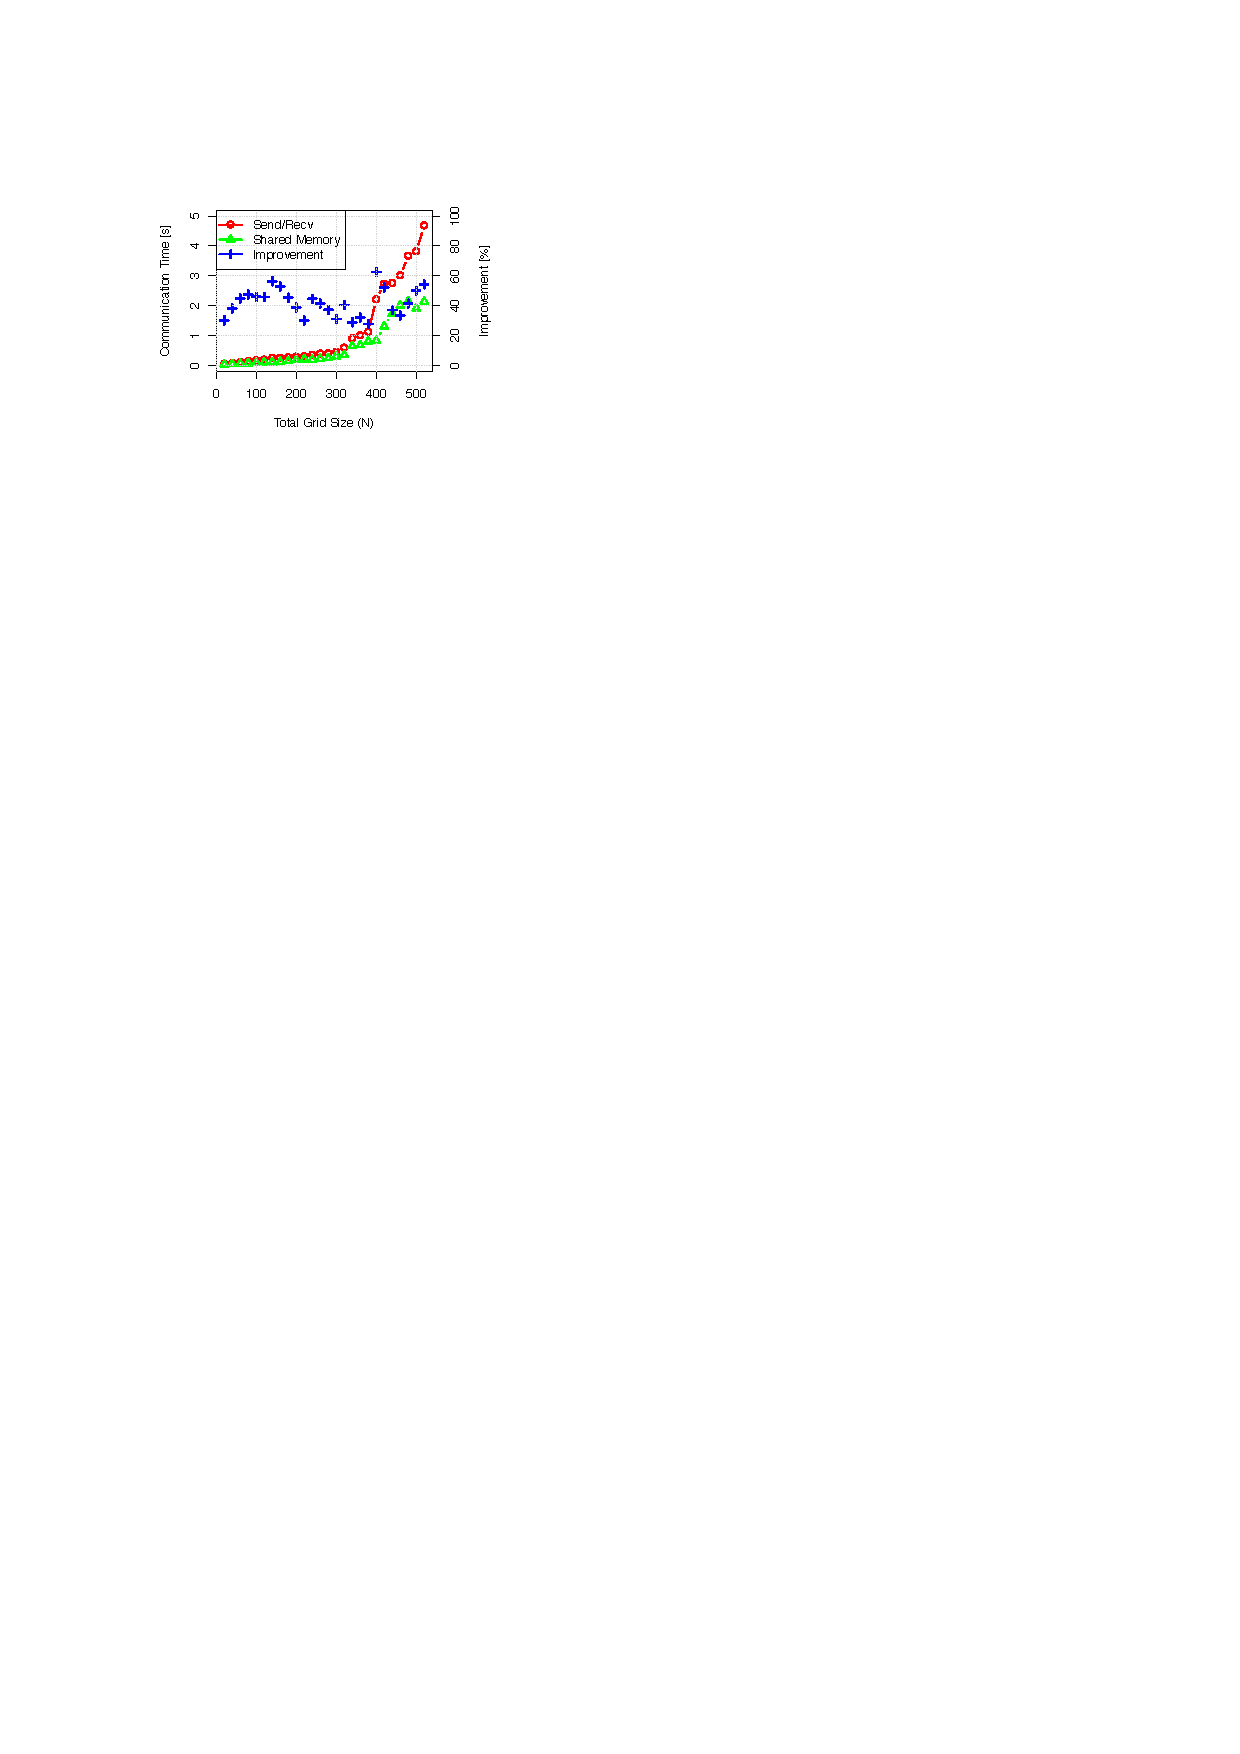
\includegraphics[scale=0.7]{./plots/Stencil_MPIMPI_CommOvhd_6core}}
   % \caption{\label{fig:stencilMPIMPIbgq}\tiny Communication and computation performance for the five-point stencil kernel.}
\end{figure}
%\column{0.3\columnwidth}
\vspace*{-.15in}
\begin{itemize}
 \item[] \footnotesize $\rightarrow$ demonstrates an average performance improvement of 40\% to the communication component of a five-point stencil solver.
\end{itemize}
%\end{columns}
\end{frame} 